\section{Parallelization and Grouping}
\label{sec:parallelization}


\noindent\textbf{Definition:} To handle large scale date, it has to be parallelized and distributed among many machines and threads. 

There is graph, and many instances of each operator. 

\begin{figure}[h]
	\centering
	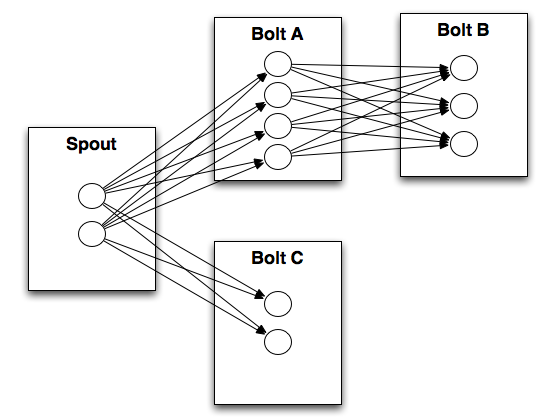
\includegraphics[width=0.45\linewidth]{grouping.png}
	\caption{ Groupings and parallelization.}
	\label{fig:grouping}
\end{figure}

\begin{figure}[h]
	\centering
	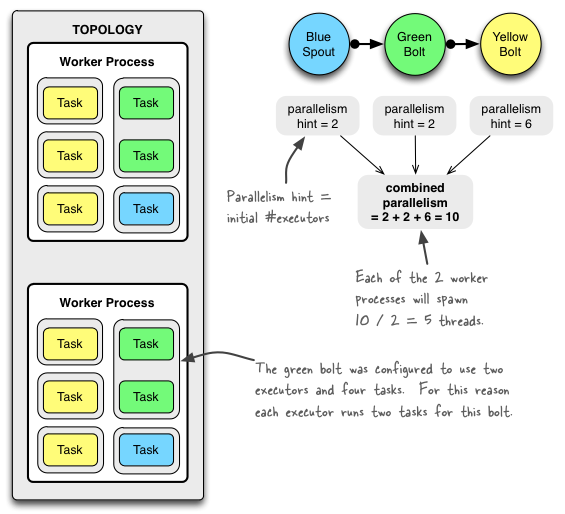
\includegraphics[width=0.45\linewidth]{jvm-task.png}
	\caption{ Distribution of operator instances}
	\label{fig:distribution}
\end{figure}


\begin{itemize}
	\item job to task partitioning
	\item data partitioning
	\item data to task mapping (groupings)
	\item thread mapping modes.
	
\end{itemize}

\noindent \textbf{\\Properties:}
\noindent \textbf{\\Solutions, trade-offs and usecases:}

\borrowed{Shuffle grouping: Tuples are randomly distributed across the bolt's tasks in a way such that each bolt is guaranteed to get an equal number of tuples.
	Fields grouping: The stream is partitioned by the fields specified in the grouping. For example, if the stream is grouped by the "user-id" field, tuples with the same "user-id" will always go to the same task, but tuples with different "user-id"'s may go to different tasks.
	Partial Key grouping: The stream is partitioned by the fields specified in the grouping, like the Fields grouping, but are load balanced between two downstream bolts, which provides better utilization of resources when the incoming data is skewed. This paper provides a good explanation of how it works and the advantages it provides.
	All grouping: The stream is replicated across all the bolt's tasks. Use this grouping with care.
	Global grouping: The entire stream goes to a single one of the bolt's tasks. Specifically, it goes to the task with the lowest id.
	None grouping: This grouping specifies that you don't care how the stream is grouped. Currently, none groupings are equivalent to shuffle groupings. Eventually though, Storm will push down bolts with none groupings to execute in the same thread as the bolt or spout they subscribe from (when possible).
	Direct grouping: This is a special kind of grouping. A stream grouped this way means that the producer of the tuple decides which task of the consumer will receive this tuple. Direct groupings can only be declared on streams that have been declared as direct streams. Tuples emitted to a direct stream must be emitted using one of the methods. A bolt can get the task ids of its consumers by either using the provided TopologyContext or by keeping track of the output of the emit method in OutputCollector (which returns the task ids that the tuple was sent to).
	Local or shuffle grouping: If the target bolt has one or more tasks in the same worker process, tuples will be shuffled to just those in-process tasks. Otherwise, this acts like a normal shuffle grouping.
}
\noindent \textbf{\\Future Direction:}  